Ebben  fejezetben külön-külön bemutatom a helpdesk alkalmazást felépítő komponenseket. Kiemelem a komponensek által megvalósított funkciókat és a megvalósítás szempontjából fontos részleteket. 


\section{Mikroszerviz infrastruktúra}

\section{Nginx}\label{sec:nginx}
Az Nginx-nek három különböző szerepe van:

\begin{itemize}
	\item a \foreignlanguage{british}{helpdesk frontend} alkalmazásszervereként működik (\ref{sec:angular}~pont),
	
	\item \foreignlanguage{british}{routing}ot valósít meg, rajta keresztül érhető el a \foreignlanguage{british}{helpdesk backend} és a \foreignlanguage{british}{Keycloak} szerviz,
	
	\item \foreignlanguage{british}{HTTP cache}-ként működik a frontend és a backend között.
\end{itemize}

A loadbalancer funkcionalitás --~mivel a docker azt natívan támogatja, így~-- a \foreignlanguage{british}{docker round-robin DNS}-én (\ref{sec:docker}) keresztül valósul meg.


\subsection{Docker konténerizáció}\label{sec:docker}
Az alakalmazás összes szolgáltatása saját docker konténerben fut. A docker konfigurációs leírása a \texttt{docker-compose.yml} állományban van. A \texttt{docker-compose} parancs ez alapján indítja el az alkalmazást, hozza létre a saját alhálózatát, valósítja meg a hálózaton belüli DNS-funkciót.

A konténerek skálázása is a dockeren keresztül (\texttt{docker-compose ----scale}) valósul meg.


\subsection{Metrikák}\label{sec:metrikak}
\Aref{sec:metrikak_tervezes} pontnak megfelelően a springes alkalmazásaim egy-egy HTTP endpointon keresztül érhetőek el a Prometheus számára (\texttt{\mbox{/actuator/proemtheus}}) és induláskor beregisztrálják magukat az Eureka\footnote{Az Eureka a Netflix által fejlesztett \emph{discovery server}. Feladata az összes kliens port és ip adatának nyilkvántartása.} szerverbe.

A Prometheus az Eurekán keresztül találja meg az instance-eket, és 15 másodpercenként összegyűjti a metrikákat. Az alkalmazások információt küldenek a Kafka konnektoraikról, REST interfészeikről és az adatbázis kapcsolataikról\footnote{HikariCP-t használok JDBC kapcsolathoz}.

A Prometheus által összegyűjtött adatokat Grafanában létrehozott --~Spring Boot és JVM metrikákat tartalmazó~--   \emph{dashboard}okon ábrázolom.


\section{E-mail kliens}
Az e-mail kliens szerepe az üzenetek küldése és fogadása egy meghatározott e-mail címről. Feladata a külső protokollok leválasztása az alkalmazásról. Irányítja és karbantartja az IMAP és SMTP szerverrel való kapcsolatot.

\Aref{fig:email-client_sequence_diagram}. ábrán látható a két irányú kommunikáció megvalósulása:
\begin{itemize}
	\item az IMAP-on keresztül fogadott e-mailt az \texttt{email.in.v1.pub} kafka topicba írja,
	\item a saját --~e-mail cím specifikus~-- topic-jából kiolvassa az üzenetet és továbbítja  az SMTP szerver felé.
\end{itemize}


\begin{figure}[hbt] 
	\centering
	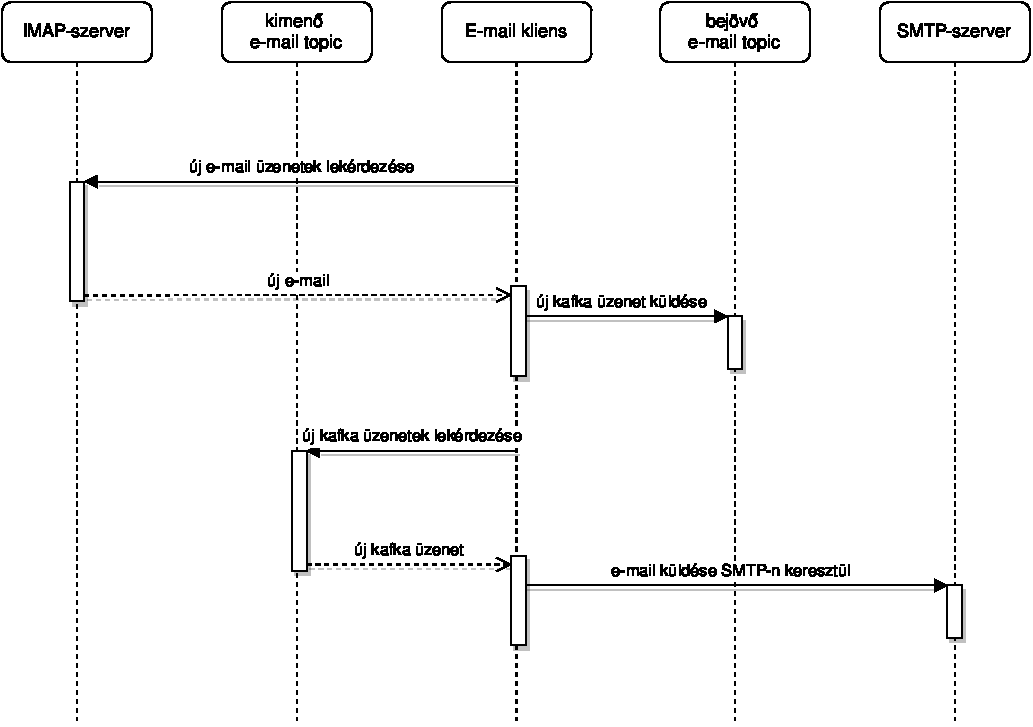
\includegraphics[width=0.85\textwidth]{email-client_sequence_diagram_drawio.pdf}
	\caption{E-mail kliens szekvencia diagramja}
	\label{fig:email-client_sequence_diagram}
	\floatfoot{Forrás: saját ábra}
\end{figure}




\subsection{E-mail szabvány}
Az elküldött üzenetek megfelelnek az \emph{rfc5322} szabványnak, különös tekintettel a 3.6.4. pontban~\cite{rfc5322_Identification_Fields} meghatározott mezőkre:

\begin{description}
	\item[Message-ID] egy globálisan egyedi azonosító ami egyértelműen azonosítja az üzenetet,
	
	\item[In-Reply-To] válasz esetén értéke eredeti üzenet \texttt{Message-ID}-ja,
	
	\item[References] azonosítja az üzenet szálat, értéke az eredeti üzenetek \texttt{Message-ID}-jai vesszővel elválasztva.
\end{description}


\section{Helpdesk backend}\label{sec:backend}
A backend felelős az e-mail szálakkal kapcsolatos üzleti feladatok ellátásáért. \Aref{fig:backend_sequence_diagram}. ábrán láthatóak a helpdesk backend funkciói:
\begin{itemize}
	\item fogadja az \texttt{email.in.v1.pub} kafka topic-ból érkező e-maileket, 
	\item kiszolgálja a frontend Nginx-en keresztül érkező kéréseit,
	\item a megfelelő kafka topic-ba írja az elküldendő üzeneteket,
	\item tárolja az e-mail szálakkal kapcsolatos adatokat.
\end{itemize}


\begin{figure}[hbt] 
	\centering
	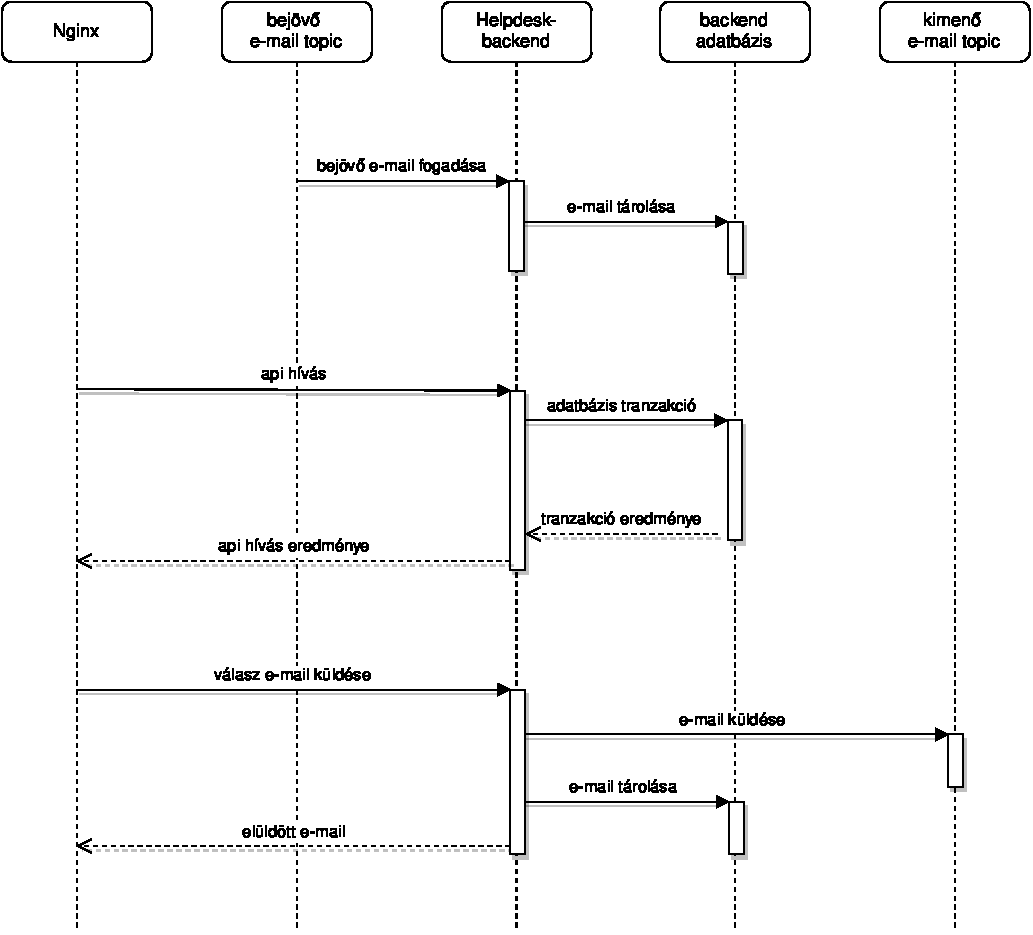
\includegraphics[width=0.85\textwidth]{backend_sequence_diagram_drawio.pdf}
	\caption{Helpdesk backend szekvencia diagramja}
	\label{fig:backend_sequence_diagram}
	\floatfoot{Forrás: saját ábra}
\end{figure}


\subsection{Spring Boot}
A forráskód Spring Boot (\ref{sec:spring_boot} pont) keretrendszerrel készült. Az elérhető modulok közül a data-jpa-t az adatbázis \texttt{repository}-jaihoz, a security-t a keycloak integrációhoz, a webet a \texttt{rest controller}ekhez, a micrometert és az actuatort a metrikák elkészítéséhez használtam.	


\subsection{Adatbázis}\label{sec:adatbazis}
A Spring kezeli --~HikariCP-n keresztül~--   a PostgreSQL adatbázishoz való kapcsolódást.
Az adatok kezelését Hibernate\footnote{A Hibernate egy JPA implementáció, ami objektum relációs leképzést valósít meg}-en keresztül, az adatbázis verziókövetését Liquibase-en (\ref{sec:liquibase} pont) keresztül valósítom meg. 

Az e-mail szálak audit információinak és verzióinak követésére a Hibernate Envers (\ref{sec:hubernate_envers} pont) eszközét használom. Az Envers a neki létrehozott táblában automatikusan követi az annotációval megjelölt entitások állapotát.

\subsection{Pesszimista konkurenciakezelés}
Pesszimista konkurenciakezelésre jó példával szolgál a Liquibase (\ref{sec:liquibase} pont) működése. 

Minden indítás során a Liquibase --~az adatbázis módosításának befejezéséig~--   zárolja a \texttt{databasechangeloglock} táblát. Így --~a várakozás miatt~-- egyszerre mindig maximum egy Liquibase példány tud elindulni és módosításokat végrehajtani.


\subsection{Optimista konkurenciakezelés}
A \ref{sec:konkurencia_kezekese} pontban ismertetett optimista konkurenciakezelést az e-mail szálak módosítása során valósítja meg a backend.

A frontend kérésére egy verziószámmal ellátott e-mail szálat küld a backend. Ezt a HTTP-protokollnak megfelelő \texttt{eTag}-et a frontend megőrzi, majd a módosítások elvégzését követően --~mint \texttt{if-match} paraméter~-- visszaküldi a módosítási kérésével együtt.

A backend összehasonlítja a módosítani kívánt erőforrás verziószámát a kérésben érkezett \texttt{if-match} verziószámmal. Ha a két szám egyezik, akkor végrehajtja a változásokat, és az erőforrás új állapota új verziószámot kap.

Ha a két verzió nem egyezik --~ami csak úgy történhet meg, ha valaki más időközben módosította a kérdéses adatot~-- akkor a tranzakció nem hajtódik végre, és a kliens egy HTTP \texttt{Conflict} hibaüzenettel értesül a történtekről. A felhasználó ilyenkor az oldal frissítése után megvizsgálja az aktuális állapotot és --~amennyiben a módosításaira még mindig szükség van --~újból kezdi a folyamatot.

\subsection{Egyéb eszközök}\label{sec:backend_egyeb_eszkozok}
A \texttt{DTO}-k és az \texttt{entity}k közötti leképezést a Mapstruct (\ref{sec:retegek_szeparalasa}) segítségével végzem. A REST \texttt{endpoint}ok dokumentációját Swagger segítségével generálom. A Swagger a felannotált osztályokból és metódusokból szabványos OpenApi dokumentációt készít. A dokumentációt \aref{appendix:openapi} függelékben csatoltam a dolgozatomhoz.



\section{Helpdesk frontend}
A frontend az e-mailek és e-mail szálakkal összefüggő üzleti feladatok megjelenítéséért felelős. A felhasználók jogosultság ellenőrzését végzi el, a bejelentkeztetésüket átirányítja a Keycloak szervernek. 


\subsection{Kommunikáció a backenddel}
A backenddel való kommunikáció HTTP protokollon keresztül zajlik, a szükséges \texttt{service} osztályokat az OpenApi dokumentációból (\ref{sec:backend_egyeb_eszkozok}) a \texttt{swagger angular generator} hozza létre.

Az aszinkron HTTP hívásokat az NgRx könyvtár alakítja adatfolyamokká. 
Az így \emph{Observable}-ként kezelt események már támogatják a stream műveleteket, megkönnyítik a filterezhetőséget és az egységes hibakezelést. 

Az NgRx használatával továbbá elkerülhetőek az aszinkron hívások mellékhatásai, és egy globális, alkalmazás szintű belső állapot hozható létre.

\subsection{Komponensek}
Az egységes megjelenés és az ismerős kinézet miatt a komponenseim alapjának az Angular Material UI könyvtárat választottam. A könyvtár népszerű az Angular fejlesztők körében, mert a leggyakrabban előforduló felhasználói igényekre elérhető benne kész, könnyen használható megoldás.

A válasz e-mail létrehozására a nyílt forráskódú Quill szövegszerkesztőt használtam, mert egyszerűen beilleszthető az Angular környezetbe, és a felhasználó számára intuitív kezelőfelülettel rendelkezik.


\subsection{Futtatási környezet}
A kész program egy egyszerű HTML, CSS és JavaScript állománnyá fordul. A körülbelül $1,5$~MB-nyi forráskódot elegendő a böngészőbe egyszer letölteni, onnantól a program a kliens oldalon fut (lásd \ref{fig:frontend_sequence_diagram} ábra). A backend felé induló REST kéréseket a webszerver (\ref{sec:nginx}) osztja szét a rendelkezésre álló példányok között.

A frontend működését, és függőségeit \aref{fig:frontend_sequence_diagram}. ábra tartalmazza.

\begin{figure}[hbp] 
	\centering
	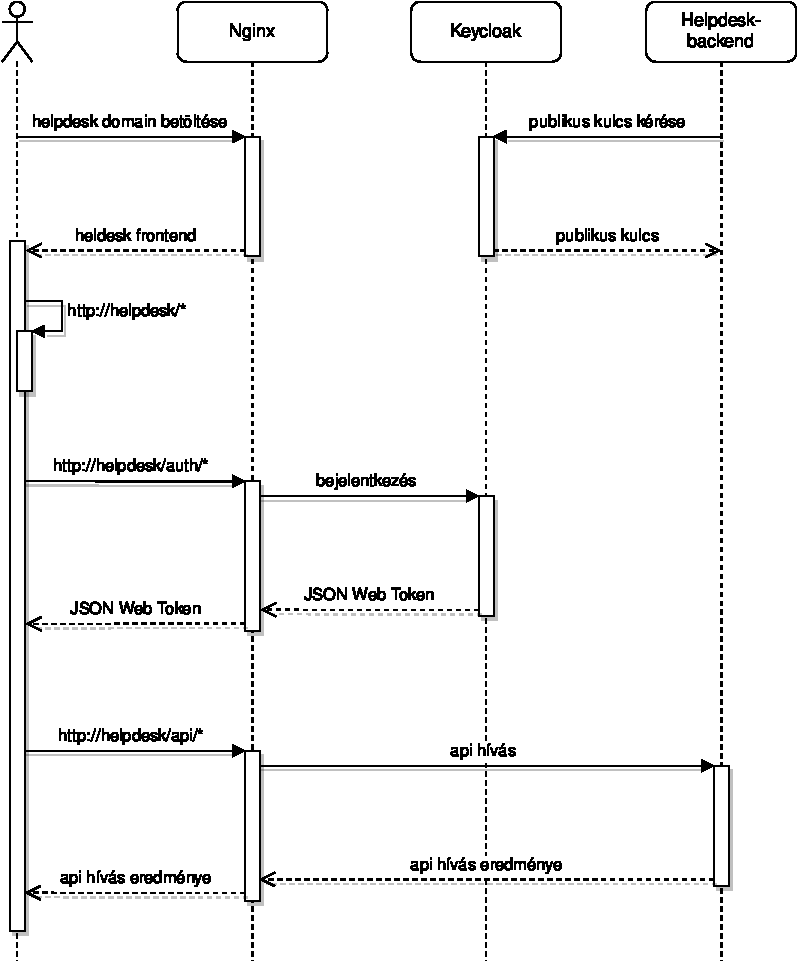
\includegraphics[width=0.85\textwidth]{frontend_sequence_diagram_drawio.pdf}
	\caption{Helpdesk frontend szekvencia diagramja}
	\label{fig:frontend_sequence_diagram}
	\floatfoot{Forrás: saját ábra}
\end{figure}


\section{Keycloak}\label{sec:keycloak}
A Keycloak egy nyílt forráskódú jogosultság- és hozzáférés-kezelő. Támogatja az LDAP-ot, SSO-t és a kétlépcsős azonosítást~\cite{Keycloak_website}. 

A helpdesk alkalmazásban feladata a felhasználók azonosítása, és adataiknak nyilvántartása. Különálló mikroszervizként, saját adatbázissal rendelkezik.

Adminisztrátor felülete segítségével nyomon követhető a különböző autentikációhoz köthető események, szerkeszthetőek az aktuálisan érvényes szerepkörök, és --~hibakezelési céllal~-- megszemélyesíthetőek a felhasználók.


\subsection{Jogosultságkezelés}\label{sec:Jogosultságkezelés}
A jogosultságokat két eltérő területre osztottam fel. A \texttt{master realm} a regisztrációért és a jogkörök kiosztásáért, míg a \texttt{helpdesk realm} az alkalmazás funkcionális (\ref{sec:tobb_felhasznalo}) feladatiért felelős.

A \texttt{helpdesk realm}on belül további két jogkört különböztetek meg. Az \texttt{admin\textunderscore user} szerepbe tartozó felhasználók képesek más e-mail szálait is kezelni, míg a csupán \texttt{regular\textunderscore user} jogkörbe tartozóak csak a saját e-mail szálaikhoz férhetnek hozzá.


\subsection{JSON Web Token}\label{sec:JWT}
A jogosultságkezelés technikai alapját az \emph{rfc7519}-es szabványban \cite{rfc7519_JSON_Web_Token} leírt JSON Web Token (JWT) adja. 

A Keycloak szervere által digitálisan aláírt token tartalmazza a felhasználó jogosultságait. A frontend minden HTTP lekérdezéshez csatolja a Keycloaktól kapott azonosítót. A backend hitelesíti a tokent a Keycloak publikus kulcsával (lásd \ref{fig:frontend_sequence_diagram} ábra), és a megfelelő jogosultság megléte esetén engedélyezi a hozzáférést az erőforráshoz.


\section{Kafka}\label{sec:implementacio_kafka}
Hogy teljesen elválasszam egymástól az e-mail klienst és a helpdesk backendet, a bejövő és kimenő e-mailek Kafka \emph{topic}-okon (\ref{sec:apache_kafka} pont) mennek keresztül. A szeparációval függetlenné teszem egymástól a két rendszer működését, ami lehetővé teszi az eltérő igénybevételnek (\ref{sec:granularitas} pont) megfelelő skálázhatóságot.

Ugyanígy, a funkciók szeparálása (\ref{sec:backend_keycloak_separation}) miatt a felhasználók adatai egy külön kafka topicban érhetőek el. Bármelyik mikroszerviznek szüksége lenne valamilyen felhasználóval kapcsolatos információra, azokat a topic végigolvasásával megkaphatja.



\section{Helpdesk backend és a Keycloak elkülönítése}\label{sec:backend_keycloak_separation}
A felhasználók adataiért a Keycloak (\ref{sec:keycloak}), az e-mail szálakért pedig a backend (\ref{sec:backend}) felelős. Az üzleti igény megköveteli hogy a felhasználók e-mail sorokhoz, és az e-mail szálak felhasználókhoz legyenek rendelve. A helpdesk backendnek éppen ezért tárolnia kell a fennálló kapcsolatokat.

A felhasználók a Keycloak felületén keresztül tudnak regisztrálni, és a személyes adataikat kezelni. A Keycloak által generált JSON Web Token (\ref{sec:JWT}) tartalmazza a felhasználók egyedi azonosítóját, a backendnek ezen az azonosítón keresztül kell a felhasználókat nyilvántartania és kiszolgálnia.

A felhasználók regisztrációja és adatainak változása --~\aref{sec:alkalmazasok_szeparalasa} pontban megismert CQRS útnak megfelelően~-- a \texttt{user.v1.pub} kafka (\ref{sec:implementacio_kafka}) topicban követhetőek nyomon.

A Keycloak Kafka integrációjának céljából hoztam létre a \texttt{keycloak-plugin} (\ref{fig:deployment_diagram} ábra) maven modult. A Keycloak esemény figyelőként működő plugin, a megfigyelt eseményekről kafka üzenetet küld a kijelölt topicba. A helpdesk backend --~a topic üzeneteit olvasva~-- tartja karban a \texttt{users} táblát (\ref{fig:basic_database_uml}, \ref{fig:extended_database_uml} ábra). Így a helpdesk backend a felhasználókról mindig aktuális információval rendelkezik.


